%!TEX root = Thesis_main.tex

\chapter{Results}
\label{chapter7}
\section{Simulations results}
\begin{floatingfigure}[r]{.33\textwidth}
	\centering
	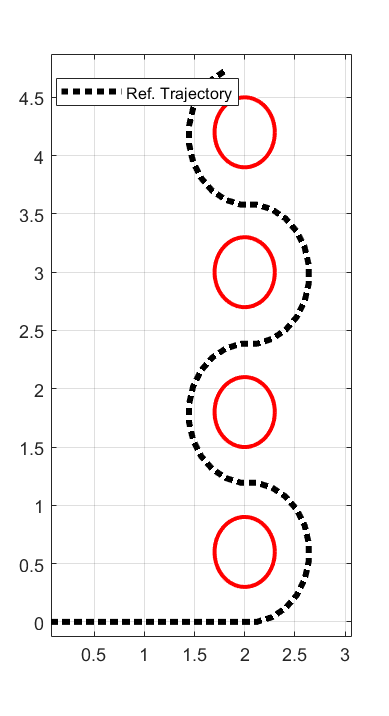
\includegraphics[scale=0.4]{traj_base_curves}
	\caption{Base trajectory for simulations: radius of the curve = 0.6m\label{traj_base_curves}}
\end{floatingfigure}
The goal of the initial simulations is to assess the actual convenience of our approach and to tune the MPC parameters and weights. Once achieved good performances with a proper set of parameters, the controller can betested with the physical system.\\
Initially some simulations with only the mobile base have been run on a trajectory with low-radius curves (in Figure \ref{traj_base_curves}), seeing the effect of different control horizon lengths and of input disturbances. This trajectory has been chosen to simulate how our controller tracks a trajectory which goes around some obstacles. No obstacle avoidance is considered in this simulation.
\begin{figure}[!h]
	\centering
	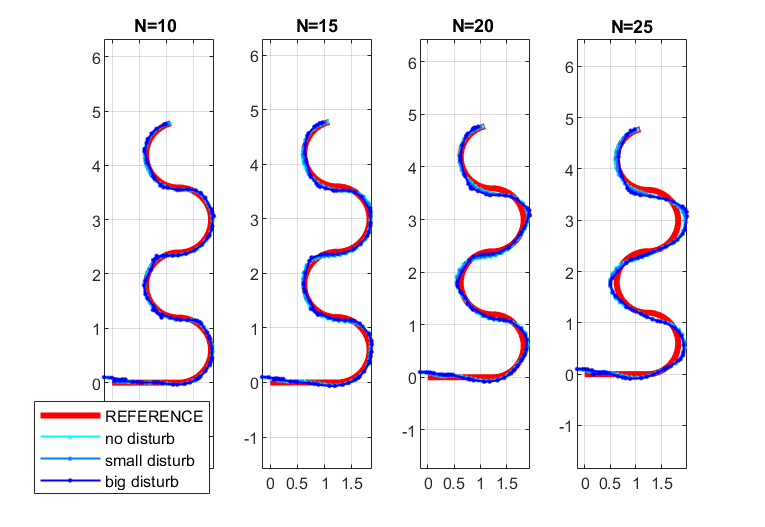
\includegraphics[scale=0.5]{base_curves}
	\caption{Mobile platform trajectories with different N}
	\label{base_curves}
\end{figure}
\begin{figure}[!h]
	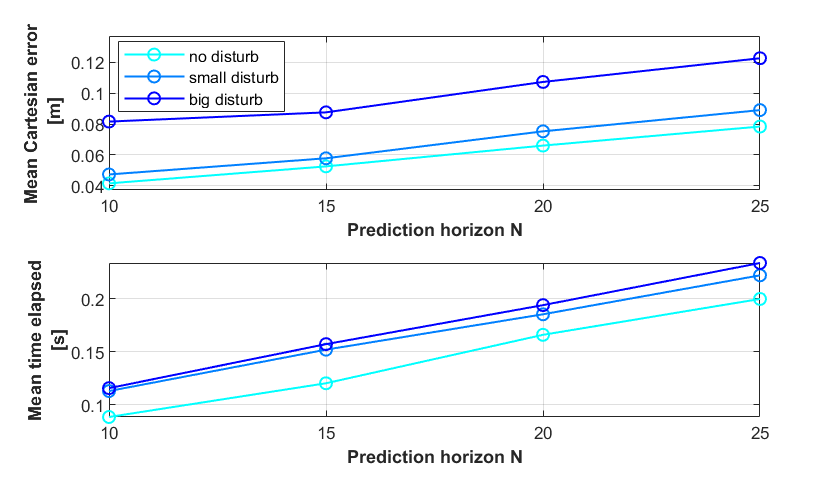
\includegraphics[scale=0.5]{base_curves_error}
	\centering
	\caption{Cartesian error and Optimization time when varying N}
	\label{base_curves_errors}
\end{figure}
\\In Figure \ref{base_curves} the trajectories that the mobile base follows are shown, considering different levels of random disturbances added to the input commands and considering different values of $N$. In Figure \ref{base_curves_errors} the relative errors and optimization times are shown. From these results we can notice that our controller is able to manage even high disturbances, but because of the limitation introduced by the parameterization of the input, it is more difficult for the optimizer to find a curve built on polynomial input commands that correctly approximates the given trajectory. This effect is even enlarged by the weighting profile of the cost function which give less importance to the accuracy of the first steps in the control horizon. Nevertheless Figure \ref{base_curves_errors} let us see that the time elapsed during the the optimization process doesn't increase exponentially like in traditional MPC, but it has just a slight increment.\\
\begin{figure}[!h]
	\centering
	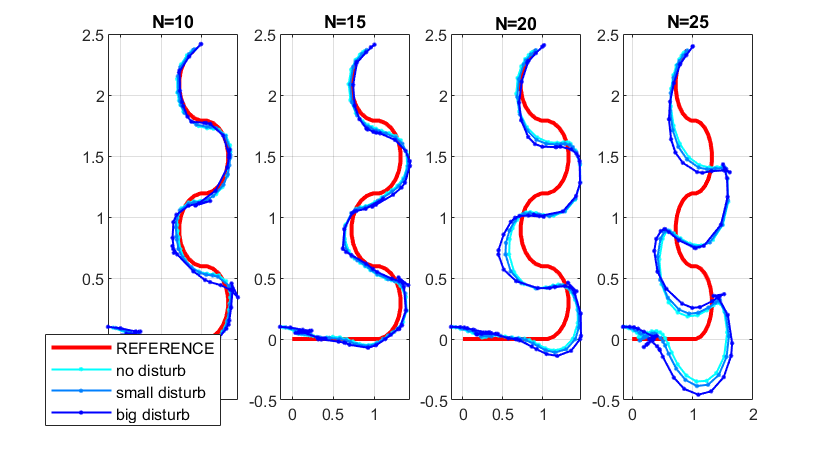
\includegraphics[scale=0.5]{base_curves2}
	\caption{Mobile platform trajectories with different N with a small-radius trajectory}
	\label{base_curves2}
\end{figure}
\begin{figure}[!h]
	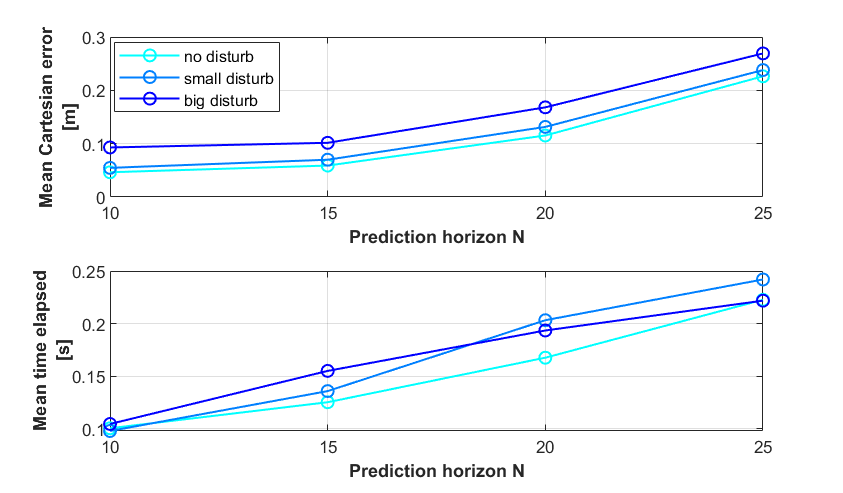
\includegraphics[scale=0.5]{base_curves_error2}
	\centering
	\caption{Cartesian error and Optimization time when varying N with a small-radius trajectory}
	\label{base_curves_errors2}
\end{figure}
To better understand the effect of a too high $N$ for complex trajectories, the same experiment has been run with a very similar trajectory but with a radius of the curves of $0.3$m instead of $0.6$m. The results of the simulations are found in Figures \ref{base_curves2} and \ref{base_curves_errors2}, where the effect of increasing $N$ is even more evident.
\begin{figure}[h!]
	\centering
	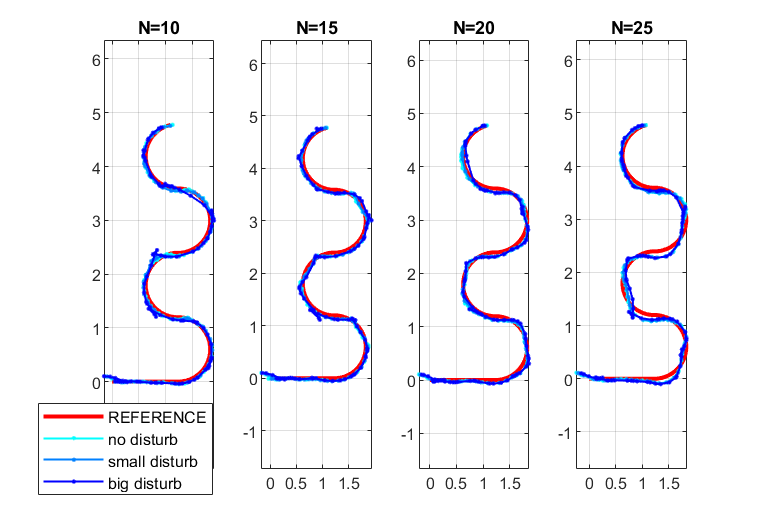
\includegraphics[scale=0.5]{base_curves3}
	\caption{Mobile platform trajectories with different N using 5th order polynomial inputs}
	\label{base_curves3}
\end{figure}
\begin{figure}[h!]
	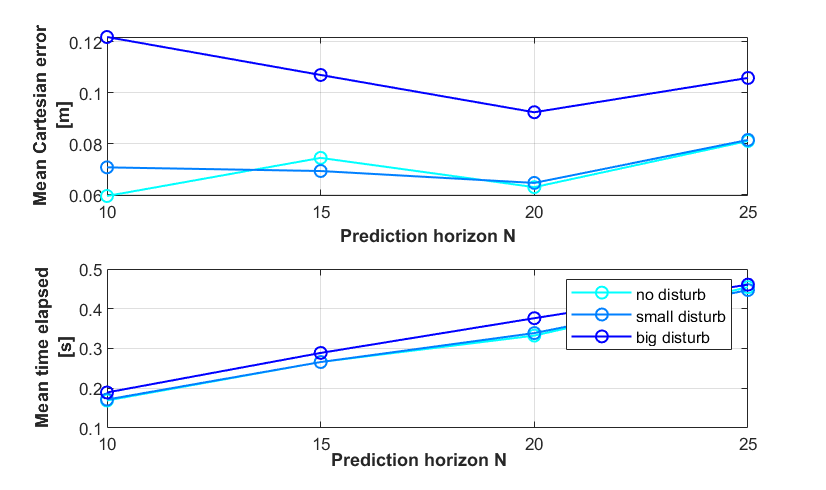
\includegraphics[scale=0.5]{base_curves_error3}
	\centering
	\caption{Cartesian error and Optimization time when varying N using 5th order polynomial inputs}
	\label{base_curves_errors3}
\end{figure}
\begin{figure}[h!]
	\centering
	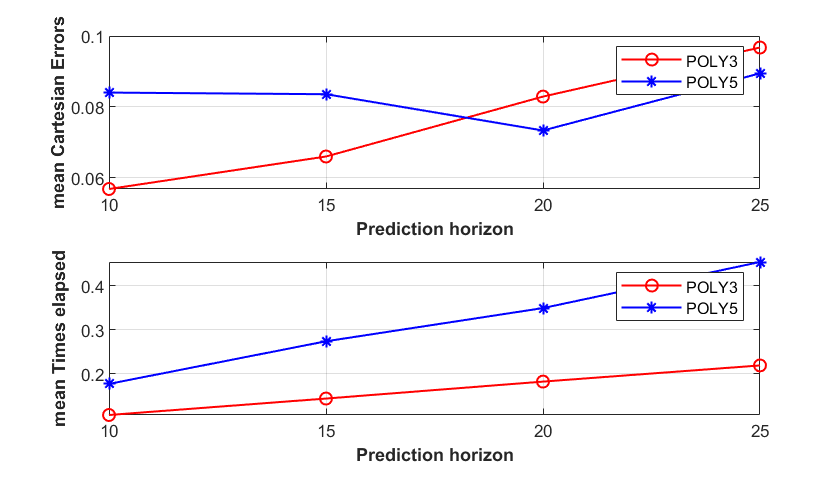
\includegraphics[scale=0.5]{base_curves_poly5}
	\caption{Comparison of errors and time of computation for 3rd and 5th order polynomial inputs}
	\label{base_curves_poly5}
\end{figure}
The previous tests have been performed describing the input commands $v$ and $\omega$ with a 3rd order polynomial. As Figures \ref{base_curves3} and \ref{base_curves_errors3} show, the effect of $N$ is lowered increasing the order of the input polynomial to 5. In Figure \ref{base_curves_poly5} a comparison in term of Cartesian error and elapsed times is shown. As was foreseeable, since the unknowns of the problem are more numerous having increased the polynomial order, the time needed for the computation of the optimization problem are higher. On the other hand, lower errors were desirable with higher order polynomials; however a better performance in this sense is reached only at high $N$, since the optimizer can now found trajectories which stay closer to the reference trajectory.
\subsection{Mobile Manipulator Handling Simulations}
The entire Mobile Manipulator has been simulated performing an EE position and orientation trajectory tracking on a sinusoidal 3D path, allowing us to more accurately tune some parameters. 
%We compared the solving times of our approach with the ones of a traditional MPC dealing with the same problem at different time horizon, in Figure \ref{solving_times}. It is easy to see the convenience of our approach, since the number of the unknowns that the optimizer has to find does not increase with $N$ and so with the dimension of the problem. In other words the mean time needed to the optimizer to solve the MPC problem stays almost constant instead of increasing exponentially.
%\begin{figure}[h!]
%	\centering
%	\includegraphics[scale=0.40]{solving_times}
%	\caption{Solving time comparison}
%	\label{solving_times}
%\end{figure}
However, from the results showed in Figure \ref{ee_tests} and from other experiments run with different time steps $T$, it can be seen that, as in previous tests, the biggest limit of this controller is that it cannot find a trajectory defined with polynomial inputs that can stay close to too complex desired trajectories during long prediction horizons

	\subsubsection{errors in tracking}
		
	\subsubsection{time elapsed}
		comparison con clasical MPC logic
	\subsubsection{J function components}

\subsection{Mobile Manipulator Grasping Simulations}

	\subsubsection{errors in tracking}
		
	\subsubsection{time elapsed}
		comparison con clasical MPC logic
	\subsubsection{J function components}
	
	\subsection{passaggio da una funz costo all'altra}

\section{Physical experiments results}

\subsection{Movement of the system toward grasping area}

	\subsubsection{errors in tracking}
		
	\subsubsection{time elapsed}
		comparison con clasical MPC logic

\subsection{Trajectory tracking in grasping operation}

	\subsubsection{errors in tracking}
		
	\subsubsection{time elapsed}
		comparison con clasical MPC logic
	\subsubsection{J function components}
